 % arara: clean: { files: [thesis.aux, thesis.bbl, thesis.blg, thesis.dvi, thesis.fdb_latexmk, thesis.fls, thesis.idx, thesis.ilg, thesis.ind, thesis.lof, thesis.log, thesis.lot, thesis.nlo, thesis.nls, thesis.out, thesis.pdf, thesis.ps, thesis.toc]}
% arara: latex:  { shell: yes }
% arara: bibtex
% arara: nomencl
% arara: latex
% arara: makeindex
% arara: latex:  { shell: yes }
% arara: dvips
% arara: ps2pdf

% ******************************* PhD Thesis Template **************************
% Please have a look at the README.md file for info on how to use the template

\documentclass[a4paper,12pt,times,numbered,print,index]{Classes/PhDThesisPSnPDF}

% ******************************************************************************
% ******************************* Class Options ********************************
% *********************** See README for more details **************************
% ******************************************************************************

% `a4paper'(The University of Cambridge PhD thesis guidelines recommends a page
% size a4 - default option) or `a5paper': A5 Paper size is also allowed as per
% the Cambridge University Engineering Deparment guidelines for PhD thesis
%
% `11pt' or `12pt'(default): Font Size 10pt is NOT recommended by the University
% guidelines
%
% `oneside' or `twoside'(default): Printing double side (twoside) or single
% side.
%
% `print': Use `print' for print version with appropriate margins and page
% layout. Leaving the options field blank will activate Online version.
%
% `index': For index at the end of the thesis
%
% `draft': For draft mode without loading any images (same as draft in book)
%
% `draftmode': Special draft mode with line numbers, images, and water mark with
% timestamp and custom text. Position of the text can also be modified.
%
% `abstract': To generate only the title page and abstract page with
% dissertation title and name, to submit to the Student Registry
%
% `chapter`: This option enables only the specified chapter and it's references
%  Useful for review and corrections.
%
% ************************* Custom Page Margins ********************************
%
% `custommargin`: Use `custommargin' in options to activate custom page margins,
% which can be defined in the preamble.tex. Custom margin will override
% print/online margin setup.
%
% *********************** Choosing the Fonts in Class Options ******************
%
% `times' : Times font with math support. (The Cambridge University guidelines
% recommend using times)
%
% `fourier': Utopia Font with Fourier Math font (Font has to be installed)
%            It's a free font.
%
% `customfont': Use `customfont' option in the document class and load the
% package in the preamble.tex
%
% default or leave empty: `Latin Modern' font will be loaded.
%
% ********************** Choosing the Bibliography style ***********************
%
% `authoryear': For author-year citation eg., Krishna (2013)
%
% `numbered': (Default Option) For numbered and sorted citation e.g., [1,5,2]
%
% `custombib': Define your own bibliography style in the `preamble.tex' file.
%              `\RequirePackage[square, sort, numbers, authoryear]{natbib}'.
%              This can be also used to load biblatex instead of natbib
%              (See Preamble)
%
% **************************** Choosing the Page Style *************************
%
% `default (leave empty)': For Page Numbers in Header (Left Even, Right Odd) and
% Chapter Name in Header (Right Even) and Section Name (Left Odd). Blank Footer.
%
% `PageStyleI': Chapter Name next & Page Number on Even Side (Left Even).
% Section Name & Page Number in Header on Odd Side (Right Odd). Footer is empty.
%
% `PageStyleII': Chapter Name on Even Side (Left Even) in Header. Section Number
% and Section Name in Header on Odd Side (Right Odd). Page numbering in footer


% ********************************** Preamble **********************************
% Preamble: Contains packages and user-defined commands and settings
% ******************************************************************************
% ****************************** Custom Margin *********************************

% Add `custommargin' in the document class options to use this section
% Set {innerside margin / outerside margin / topmargin / bottom margin}  and
% other page dimensions
\ifsetCustomMargin
  \RequirePackage[left=37mm,right=30mm,top=35mm,bottom=30mm]{geometry}
  \setFancyHdr % To apply fancy header after geometry package is loaded
\fi

% *****************************************************************************
% ******************* Fonts (like different typewriter fonts etc.)*************

% Add `customfont' in the document class option to use this section

\ifsetCustomFont
  % Set your custom font here and use `customfont' in options. Leave empty to
  % load computer modern font (default LaTeX font).
  \RequirePackage{helvet}
\fi

% *****************************************************************************
% **************************** Custom Packages ********************************

% ************************* Algorithms and Pseudocode **************************

\usepackage{algpseudocode}


% ********************Captions and Hyperreferencing / URL **********************

% Captions: This makes captions of figures use a boldfaced small font.
%\RequirePackage[small,bf]{caption}

\RequirePackage[labelsep=space,tableposition=top]{caption}
\renewcommand{\figurename}{Fig.} %to support older versions of captions.sty


% *************************** Graphics and figures *****************************

%\usepackage{rotating}
%\usepackage{wrapfig}

% Uncomment the following two lines to force Latex to place the figure.
% Use [H] when including graphics. Note 'H' instead of 'h'
%\usepackage{float}
%\restylefloat{figure}

% Subcaption package is also available in the sty folder you can use that by
% uncommenting the following line
% This is for people stuck with older versions of texlive
%\usepackage{sty/caption/subcaption}
\usepackage{subcaption}

% ********************************** Tables ************************************
\usepackage{booktabs} % For professional looking tables
\usepackage{multirow}

%\usepackage{multicol}
%\usepackage{longtable}
%\usepackage{tabularx}


% ***************************** Math and SI Units ******************************

\usepackage{amsfonts}
\usepackage{amsmath}
\usepackage{amssymb}
\usepackage{siunitx} % use this package module for SI units


% ******************************* Line Spacing *********************************

% Choose linespacing as appropriate. Default is one-half line spacing as per the
% University guidelines

% \doublespacing
% \onehalfspacing
% \singlespacing


% ************************ Formatting / Footnote *******************************

% Don't break enumeration (etc.) across pages in an ugly manner (default 10000)
%\clubpenalty=500
%\widowpenalty=500

%\usepackage[perpage]{footmisc} %Range of footnote options


% *****************************************************************************
% *************************** Bibliography  and References ********************

%\usepackage{cleveref} %Referencing without need to explicitly state fig /table

% Add `custombib' in the document class option to use this section
\ifuseCustomBib
   \RequirePackage[square, sort, numbers, authoryear]{natbib} % CustomBib

% If you would like to use biblatex for your reference management, as opposed to the default `natbibpackage` pass the option `custombib` in the document class. Comment out the previous line to make sure you don't load the natbib package. Uncomment the following lines and specify the location of references.bib file

%\RequirePackage[backend=biber, style=numeric-comp, citestyle=numeric, sorting=nty, natbib=true]{biblatex}
%\bibliography{References/references} %Location of references.bib only for biblatex

\fi

% changes the default name `Bibliography` -> `References'
\renewcommand{\bibname}{References}


% *****************************************************************************
% *************** Changing the Visual Style of Chapter Headings ***************
% This section on visual style is from https://github.com/cambridge/thesis

% Uncomment the section below. Requires titlesec package.

%\RequirePackage{titlesec}
%\newcommand{\PreContentTitleFormat}{\titleformat{\chapter}[display]{\scshape\Large}
%{\Large\filleft{\chaptertitlename} \Huge\thechapter}
%{1ex}{}
%[\vspace{1ex}\titlerule]}
%\newcommand{\ContentTitleFormat}{\titleformat{\chapter}[display]{\scshape\huge}
%{\Large\filleft{\chaptertitlename} \Huge\thechapter}{1ex}
%{\titlerule\vspace{1ex}\filright}
%[\vspace{1ex}\titlerule]}
%\newcommand{\PostContentTitleFormat}{\PreContentTitleFormat}
%\PreContentTitleFormat


% ******************************************************************************
% ************************* User Defined Commands ******************************
% ******************************************************************************

% *********** To change the name of Table of Contents / LOF and LOT ************

%\renewcommand{\contentsname}{My Table of Contents}
%\renewcommand{\listfigurename}{My List of Figures}
%\renewcommand{\listtablename}{My List of Tables}


% ********************** TOC depth and numbering depth *************************

\setcounter{secnumdepth}{2}
\setcounter{tocdepth}{2}


% ******************************* Nomenclature *********************************

% To change the name of the Nomenclature section, uncomment the following line

%\renewcommand{\nomname}{Symbols}


% ********************************* Appendix ***********************************

% The default value of both \appendixtocname and \appendixpagename is `Appendices'. These names can all be changed via:

%\renewcommand{\appendixtocname}{List of appendices}
%\renewcommand{\appendixname}{Appndx}

% ******************************** Draft Mode **********************************

% Uncomment to disable figures in `draftmode'
%\setkeys{Gin}{draft=true}  % set draft to false to enable figures in `draft'

% These options are active only during the draft mode
% Default text is "Draft"
%\SetDraftText{DRAFT}

% Default Watermark location is top. Location (top/bottom)
%\SetDraftWMPosition{bottom}

% Draft Version - default is v1.0
%\SetDraftVersion{v1.1}

% Draft Text grayscale value (should be between 0-black and 1-white)
% Default value is 0.75
%\SetDraftGrayScale{0.8}


%% Todo notes functionality
%% Uncomment the following lines to have todonotes.

%\ifsetDraft
%	\usepackage[colorinlistoftodos]{todonotes}
%	\newcommand{\mynote}[1]{\todo[author=kks32,size=\small,inline,color=green!40]{#1}}
%\else
%	\newcommand{\mynote}[1]{}
%	\newcommand{\listoftodos}{}
%\fi

% Example todo: \mynote{Hey! I have a note}


% ************************ Thesis Information & Meta-data **********************
% Thesis title and author information, refernce file for biblatex
% ************************ Thesis Information & Meta-data **********************
%% The title of the thesis
\title{Machine Learning methods for Thin Vessel Segmentation}
%\texorpdfstring is used for PDF metadata. Usage:
%\texorpdfstring{LaTeX_Version}{PDF Version (non-latex)} eg.,
%\texorpdfstring{$sigma$}{sigma}

%% Subtitle (Optional)
\subtitle{in Fundus Images}

%% The full name of the author
\author{Kushal Khandelwal}

%% Department (eg. Department of Engineering, Maths, Physics)
%\dept{Department of Engineering}

%% University and Crest
\university{Birla Institute of Technology and Science,Pilani}
\crest{
\includegraphics[width=0.25\textwidth]{University_Crest}}

%% You can redefine the submission text:
% Default as per the University guidelines:
% ``This dissertation is submitted for the degree of''
\renewcommand{\submissiontext}{This thesis is submitted in requirements of the course BITS C421T}

%% Full title of the Degree
%\degreetitle{Doctor of Philosophy}

%% College affiliation (optional)
%\college{King's College}

%% Submission date
% Default is set as {\monthname[\the\month]\space\the\year}
\degreedate{May 2015} 

%% Meta information
\subject{LaTeX} \keywords{{LaTeX} {Master Thesis} {Engineering} {Birla Institute of Technology and Science, Pilani}}


% ***************************** Abstract Separate ******************************
% To printout only the titlepage and the abstract with the PhD title and the
% author name for submission to the Student Registry, use the `abstract' option in
% the document class.

\ifdefineAbstract
 \pagestyle{empty}
 \includeonly{Declaration/declaration, Abstract/abstract}
\fi

% ***************************** Chapter Mode ***********************************
% The chapter mode allows user to only print particular chapters with references
% Title, Contents, Frontmatter are disabled by default
% Useful option to review a particular chapter or to send it to supervisior.
% To use choose `chapter' option in the document class

\ifdefineChapter
 \includeonly{Chapter3/chapter3}
\fi

% ******************************** Front Matter ********************************
\begin{document}

\frontmatter

\begin{titlepage}
  \maketitle
\end{titlepage}


%% ******************************* Thesis Dedidcation ********************************

\begin{dedication} 

I would like to dedicate this thesis to my loving parents and my w \dots

\end{dedication}


%% ******************************* Thesis Declaration ***************************

\begin{declaration}

I hereby declare that except where specific reference is made to the work of 
others, the contents of this dissertation are original and have not been 
submitted in whole or in part for consideration for any other degree or 
qualification in this, or any other university. This dissertation is my own 
work and contains nothing which is the outcome of work done in collaboration 
with others, except as specified in the text and Acknowledgements. This 
dissertation contains fewer than 65,000 words including appendices, 
bibliography, footnotes, tables and equations and has fewer than 150 figures.

% Author and date will be inserted automatically from thesis.tex \author \degreedate

\end{declaration}


% ************************** Thesis Acknowledgements **************************

\begin{acknowledgements}      

First, I would like to thank my thesis advisor Professor Fred Hamprecht, whose constant guidance and support has helped me to learn a lot while working towards the thesis. I would like to thank him for providing me this opportunity write my thesis in his group. I would also like to express my sincere gratitude to my mentor Dr. Ferran Diego, who has always been an excellent mentor an a guide. His constant feedback during the entire duration of thesis has helped me to complete my thesis in Heidelberg. I would also like to thank my co-mentor Dr. Melih Kandemir for his valuable feedback.\\

I also want to thank all the current and former member of the Multidimensional Image Processing group for those invaluavle discussions and suggestions and  for making the time at Heidelberg Collaboratory for Image Processing much more fun.
I would also like to thank my on campus supervisor in India Dr. Sukanta Mondal, for helping me throughout the duration of thesis at various stages.\\

I would like to thank my parents and my sister, for being with me all the time and providing me with the constant pillar of support and who kept me motivated during the entire duration of my work.\\

Last but not the least, I would like to thank the coordinators of Erasmus Mundus mobility with Asia (EMMA) , for providing the financila suppoer and making this exchange possible. 


\end{acknowledgements}

% $Log: abstract.tex,v $
% Revision 1.1  93/05/14  14:56:25  starflt
% Initial revision
% 
% Revision 1.1  90/05/04  10:41:01  lwvanels
% Initial revision
% 
%
%% The text of your abstract and nothing else (other than comments) goes here.
%% It will be single-spaced and the rest of the text that is supposed to go on
%% the abstract page will be generated by the abstractpage environment.  This
%% file should be \input (not \include 'd) from cover.tex.
In this thesis, I designed and implemented a compiler which performs
optimizations that reduce the number of low-level floating point operations
necessary for a specific task; this involves the optimization of chains of
floating point operations as well as the implementation of a ``fixed'' point
data type that allows some floating point operations to simulated with integer
arithmetic.  The source language of the compiler is a subset of C, and the
destination language is assembly language for a micro-floating point CPU.  An
instruction-level simulator of the CPU was written to allow testing of the
code.  A series of test pieces of codes was compiled, both with and without
optimization, to determine how effective these optimizations were.


% *********************** Adding TOC and List of Figures ***********************

\tableofcontents

\listoffigures

\listoftables

% \printnomencl[space] space can be set as 2em between symbol and description
%\printnomencl[3em]

\printnomencl

% ******************************** Main Matter *********************************
\mainmatter

%*******************************************************************************
%*********************************** First Chapter *****************************
%*******************************************************************************

\chapter{Introdcution}  %Title of the First Chapter

\ifpdf
    \graphicspath{{Chapter1/Figs/Raster/}{Chapter1/Figs/PDF/}{Chapter1/Figs/}}
\else
    \graphicspath{{Chapter1/Figs/Vector/}{Chapter1/Figs/}}
\fi


%********************************** %First Section  **************************************
\section{What is loren ipsum? Title with math \texorpdfstring{$\sigma$}{[sigma]}} %Section - 1.1 

Lorem Ipsum is simply dummy text of the printing and typesetting industry (see 
Section~\ref{section1.3}). Lorem Ipsum~\citep{Aup91} has been the industry's 
standard dummy text ever since the 1500s, when an unknown printer took a galley 
of type and scrambled it to make a type specimen book. It has survived not only 
five centuries, but also the leap into electronic typesetting, remaining 
essentially unchanged. It was popularised in the 1960s with the release of 
Letraset sheets containing Lorem Ipsum passages, and more recently with desktop 
publishing software like Aldus PageMaker including versions of Lorem 
Ipsum~\citep{AAB95,Con90,LM65}.

The most famous equation in the world: $E^2 = (m_0c^2)^2 + (pc)^2$, which is 
known as the \textbf{energy-mass-momentum} relation as an in-line equation.

A {\em \LaTeX{} class file}\index{\LaTeX{} class file@LaTeX class file} is a file, which holds style information for a particular \LaTeX{}.


\begin{align}
CIF: \hspace*{5mm}F_0^j(a) = \frac{1}{2\pi \iota} \oint_{\gamma} \frac{F_0^j(z)}{z - a} dz
\end{align}

\nomenclature[z-cif]{$CIF$}{Cauchy's Integral Formula}                                % first letter Z is for Acronyms 
\nomenclature[a-F]{$F$}{complex function}                                                   % first letter A is for Roman symbols
\nomenclature[g-p]{$\pi$}{ $\simeq 3.14\ldots$}                                             % first letter G is for Greek Symbols
\nomenclature[g-i]{$\iota$}{unit imaginary number $\sqrt{-1}$}                      % first letter G is for Greek Symbols
\nomenclature[g-g]{$\gamma$}{a simply closed curve on a complex plane}  % first letter G is for Greek Symbols
\nomenclature[x-i]{$\oint_\gamma$}{integration around a curve $\gamma$} % first letter X is for Other Symbols
\nomenclature[r-j]{$j$}{superscript index}                                                       % first letter R is for superscripts
\nomenclature[s-0]{$0$}{subscript index}                                                        % first letter S is for subscripts


%********************************** %Second Section  *************************************
\section{Why do we use loren ipsum?} %Section - 1.2


It is a long established fact that a reader will be distracted by the readable content of a page when looking at its layout. The point of using Lorem Ipsum is that it has a more-or-less normal distribution of letters, as opposed to using `Content here, content here', making it look like readable English. Many desktop publishing packages and web page editors now use Lorem Ipsum as their default model text, and a search for `lorem ipsum' will uncover many web sites still in their infancy. Various versions have evolved over the years, sometimes by accident, sometimes on purpose (injected humour and the like).

%********************************** % Third Section  *************************************
\section{Where does it come from?}  %Section - 1.3 
\label{section1.3}

Contrary to popular belief, Lorem Ipsum is not simply random text. It has roots in a piece of classical Latin literature from 45 BC, making it over 2000 years old. Richard McClintock, a Latin professor at Hampden-Sydney College in Virginia, looked up one of the more obscure Latin words, consectetur, from a Lorem Ipsum passage, and going through the cites of the word in classical literature, discovered the undoubtable source. Lorem Ipsum comes from sections 1.10.32 and 1.10.33 of "de Finibus Bonorum et Malorum" (The Extremes of Good and Evil) by Cicero, written in 45 BC. This book is a treatise on the theory of ethics, very popular during the Renaissance. The first line of Lorem Ipsum, "Lorem ipsum dolor sit amet..", comes from a line in section 1.10.32.

The standard chunk of Lorem Ipsum used since the 1500s is reproduced below for those interested. Sections 1.10.32 and 1.10.33 from ``de Finibus Bonorum et Malorum" by Cicero are also reproduced in their exact original form, accompanied by English versions from the 1914 translation by H. Rackham

``Lorem ipsum dolor sit amet, consectetur adipisicing elit, sed do eiusmod tempor incididunt ut labore et dolore magna aliqua. Ut enim ad minim veniam, quis nostrud exercitation ullamco laboris nisi ut aliquip ex ea commodo consequat. Duis aute irure dolor in reprehenderit in voluptate velit esse cillum dolore eu fugiat nulla pariatur. Excepteur sint occaecat cupidatat non proident, sunt in culpa qui officia deserunt mollit anim id est laborum."

Section 1.10.32 of ``de Finibus Bonorum et Malorum", written by Cicero in 45 BC: ``Sed ut perspiciatis unde omnis iste natus error sit voluptatem accusantium doloremque laudantium, totam rem aperiam, eaque ipsa quae ab illo inventore veritatis et quasi architecto beatae vitae dicta sunt explicabo. Nemo enim ipsam voluptatem quia voluptas sit aspernatur aut odit aut fugit, sed quia consequuntur magni dolores eos qui ratione voluptatem sequi nesciunt. Neque porro quisquam est, qui dolorem ipsum quia dolor sit amet, consectetur, adipisci velit, sed quia non numquam eius modi tempora incidunt ut labore et dolore magnam aliquam quaerat voluptatem. Ut enim ad minima veniam, quis nostrum exercitationem ullam corporis suscipit laboriosam, nisi ut aliquid ex ea commodi consequatur? Quis autem vel eum iure reprehenderit qui in ea voluptate velit esse quam nihil molestiae consequatur, vel illum qui dolorem eum fugiat quo voluptas nulla pariatur?"

1914 translation by H. Rackham: ``But I must explain to you how all this mistaken idea of denouncing pleasure and praising pain was born and I will give you a complete account of the system, and expound the actual teachings of the great explorer of the truth, the master-builder of human happiness. No one rejects, dislikes, or avoids pleasure itself, because it is pleasure, but because those who do not know how to pursue pleasure rationally encounter consequences that are extremely painful. Nor again is there anyone who loves or pursues or desires to obtain pain of itself, because it is pain, but because occasionally circumstances occur in which toil and pain can procure him some great pleasure. To take a trivial example, which of us ever undertakes laborious physical exercise, except to obtain some advantage from it? But who has any right to find fault with a man who chooses to enjoy a pleasure that has no annoying consequences, or one who avoids a pain that produces no resultant pleasure?"

Section 1.10.33 of ``de Finibus Bonorum et Malorum", written by Cicero in 45 BC: ``At vero eos et accusamus et iusto odio dignissimos ducimus qui blanditiis praesentium voluptatum deleniti atque corrupti quos dolores et quas molestias excepturi sint occaecati cupiditate non provident, similique sunt in culpa qui officia deserunt mollitia animi, id est laborum et dolorum fuga. Et harum quidem rerum facilis est et expedita distinctio. Nam libero tempore, cum soluta nobis est eligendi optio cumque nihil impedit quo minus id quod maxime placeat facere possimus, omnis voluptas assumenda est, omnis dolor repellendus. Temporibus autem quibusdam et aut officiis debitis aut rerum necessitatibus saepe eveniet ut et voluptates repudiandae sint et molestiae non recusandae. Itaque earum rerum hic tenetur a sapiente delectus, ut aut reiciendis voluptatibus maiores alias consequatur aut perferendis doloribus asperiores repellat."

1914 translation by H. Rackham: ``On the other hand, we denounce with righteous indignation and dislike men who are so beguiled and demoralized by the charms of pleasure of the moment, so blinded by desire, that they cannot foresee the pain and trouble that are bound to ensue; and equal blame belongs to those who fail in their duty through weakness of will, which is the same as saying through shrinking from toil and pain. These cases are perfectly simple and easy to distinguish. In a free hour, when our power of choice is untrammelled and when nothing prevents our being able to do what we like best, every pleasure is to be welcomed and every pain avoided. But in certain circumstances and owing to the claims of duty or the obligations of business it will frequently occur that pleasures have to be repudiated and annoyances accepted. The wise man therefore always holds in these matters to this principle of selection: he rejects pleasures to secure other greater pleasures, or else he endures pains to avoid worse pains."

%*******************************************************************************
%****************************** Second Chapter *********************************
%*******************************************************************************

\chapter{Background and Literature Review}

\ifpdf
    \graphicspath{{Chapter2/Figs/Raster/}{Chapter2/Figs/PDF/}{Chapter2/Figs/}}
\else
    \graphicspath{{Chapter2/Figs/Vector/}{Chapter2/Figs/}}
\fi

This chapter aims to provide the basic background knowledge to understand the work of thesis. Clustering algortighm and Dictionary Learning algortihms are discusses. We further discuss the various evaluation measures.
\section[Machine Learning]{Machine Learning}

Machine learning is the study dealing with the process to learn characteristic information from data. Given some data, $ X $ , a machine learning algorithm learns a function $ f(x) $ which maps the input to an output variable $y$ . The learnt model than can be used to make predictions on previously unseen data $X'$. The aim of a machine learning algorithm is to learn a generalized model which can make the best possible prediction on the new previously unseen data.

To train the algorithm, it is fed with data points (known as training observations/instances). The data points in the set are each described by a set of features, know as feature vectors. These descriptors can be learned from the data or can be computed for each instance. As an example, supppose we have a set of patches from an image as our data points. Descritors denote the key properties of data points.

Let $X =\{x_1,x_2,... x_n\} \in R^{m x n}$ be a set of images patches with dimesnsions ${m x n}$. The feature vector describing these data points can than be denoted as
\begin{equation*}
X = \begin{pmatrix}
x_{1,1} & x_{1,2} & \cdots & x_{1,n} \\
x_{2,1} & x_{2,2} & \cdots & x_{2,n} \\
\vdots  & \vdots  & \ddots & \vdots  \\
x_{m,1} & x_{m,2} & \cdots & x_{m,n}
\end{pmatrix}
\end{equation*}
Here each row of the matrix dentoes individual data points and ${x_{i,j}}$ are the gray scale intensities of each pixel of the given patch $x_i$.





Depending on whether the data is labelled or unlabelled, the machine learning algorithms can be divided into two types namely :
\begin{enumerate}
	\item Supervised Learning Algorithms
	\item Unsupervised Learning Algorithms
\end{enumerate}

\subsection{Supervised Learning}
Give a training set of labelled data, supervised learning algorithims fit a model to the training set with the aim of predciting the unknown labels for the test instances ( observations). During the training phase, the algorithms learns the unkown parameters for the model.

[Describe the process]

[Example of a learning algorithm]

\subsection{Unsupervised Learning}

In unsupervised learning settings, the task is to find group relations between instances of the unlabeled training dataset with a subsequent aim of categorizing or clustering the data. The algorithm aims to understand the general properties/structure in the dataset.

[Explain the method]

\section{Clustering}
A cluster is collection of data points grouped together on basis of some common properties.The data objects or points within a cluster are similar to each other, whereas the points in different groups are disimilar.

The process of partioning of data points into smaller groups (called as clusters) with the aim to minimize the intra cluster variance and maximize the inter cluster variance. The grouping of data points is based on the similarity or disimilarity of the objects as described by their properties or features. Clustering data objects create subspaces within the data.

[For example, given a toy dataset with 10 data points]


Similarity or disimilarity between two objectives can be very subjective and hence various measures are used to describe them quantitatively with distance measure being the most common.The distance measure is used to specify the distance between two objects and can be used to create a distance matrix called as similarity/disimilarity matrix. The most used distance metric is the Minkowski Distances.

[Minkowski distances]

As the data labels are unknown,cluster analysis is known as an unsupervised method of data partionining.This is contast to classification where the data can be partitioned on the basis of their class labels. Thus, clustering segments the data on the basis of the properties of the objects within the dataset and finds previously unkown grouping within the data.

The distance based clustering algorithms can be divided into two types namely Partioning based and Hiearchical methods.

We look into these different types of Clustering methods.

\subsection{K-Means Clustering}
In this section we look into the K-Means clustering algorithm. We assume that the number of clusters 'K' is given and we use it to initiate our clustering algorirthm. 

We are give a dataset D with n objects. Each n object in the dataset is described by a feature vector of length m. The feature vector can be anything which can represent the datapoint. For examples, for an image the feature vector can be grayscale values at every pixel. The aim of the clustering algorithm is to partition the the dataset D[m x n] into 'K' clusters while optimizing an objective function. The clusters are formed so as to the objects within the same cluster are similar and disimilar to objects in other clusters.


K-Means is a centroid based partioning method I.e the centroid of the cluster is the representative data point for the cluster. The centorid of the cluster is defined by the mean of all the data points within the cluster.

Give a dataset D with n objects in the Eucledian space, the aim is to partition the dataset into k cluster C1,C2...Ck susch that Ci subset of D and Ci Cj is nil. That is each point withing the dataset is exclusive to one cluster.
Each of the clusters Ci is represented by its centroid ci. Each cluster is consists of p points and the distance between the point p and the cluster representative ci is defined as dist(p,ci). If the data points are in m dimensional , then the distance is defined as
[eucledian distance]

The clustering algorithm optimizes the inter cluster variation, this is the Sum of Squared Error(SSE) between the data points in the cluster and the centroid. 
The SSE  is defined as 

Error = 

Algorithm

Algorithm

\section{Decompostion Methods}

\subsection{PCA}
\subsection{Matrix Factorization}

\section{Dictionary Learning}
\subsection{Sparse Coding}

\section{Preprocessing Methods}
\subsection{Normalization}
\subsection{CLAHE}

\section{Evaluation}
\chapter{Framework}

% **************************** Define Graphics Path **************************
\ifpdf
    \graphicspath{{Chapter3/Figs/Raster/}{Chapter3/Figs/PDF/}{Chapter3/Figs/}}
\else
    \graphicspath{{Chapter3/Figs/Vector/}{Chapter3/Figs/}}
\fi
The chapter aims to present the basic framework for our vessel segmentation algorithm.
The chapter is divided into 4 parts. In the first part we discuss the basic framework of our algorithm. Part 2 and Part3 talk about the various preprocessing methods and how the methods was applied to our problem.
\section{Vessel segmentation Framework}
The image segmentation framework takes as its input a list of fundus images, $I = (I^{(1)},I^{(2)}....., I^{(n)} )$  and their correspoding ground truth segmentation maps  $S = (S^{(1)},S^{(2)}....., S^{(n)} )$. The fundus images $I^n$ can be grayscale or RGB color images. For each n, $S^n$ ,the binary segmentation map is of the same size as of $I^n$. For a given fundus image, $I^n$, let $I^n(x,y)$ denote the pixel value at position (x,y) and $S^n(x,y)$ denotes the corresponding pixel in the segmentation map $S^n$. The pixels in segmentation map take either a value of 1 or 0 denoting the presenece or absence of vessel respectively.

\begin{figure}
	\centering
	\begin{subfigure}[b]{0.45\textwidth}
		\centering
		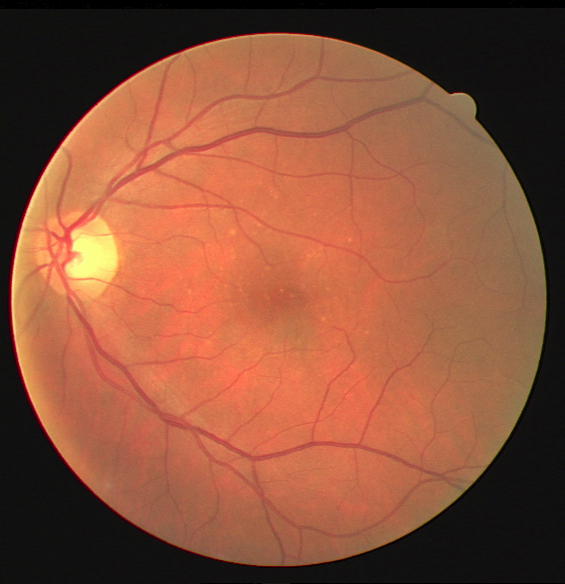
\includegraphics[width=\textwidth]{fundusimage}
		\caption{Fundus Image}
		\label{fig:fundusex}
	\end{subfigure}
	\hfill
	\begin{subfigure}[b]{0.45\textwidth}
		\centering
		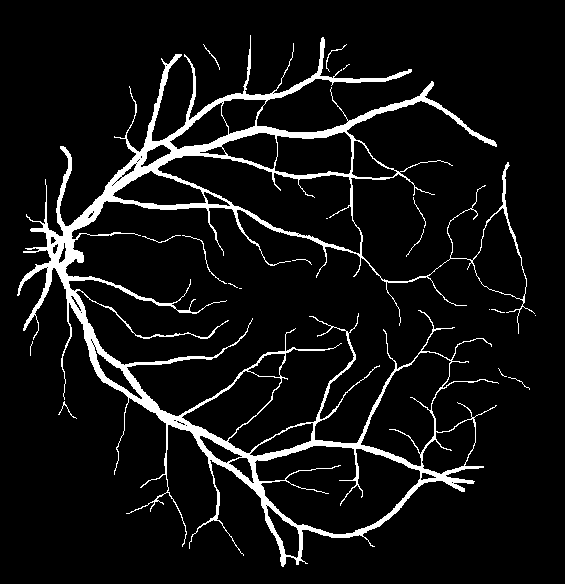
\includegraphics[width=\textwidth]{fundusimageseg}
		\caption{Segmented Vessels}
		\label{fig:fundusex seg}
	\end{subfigure}
	\caption{Fundus Image and its segmentation}
	\label{fig:fundus example}
\end{figure}


For clarity and simplicity, the fundus images will be referred as I and the corresponding segmentation image as S. Fig~\ref{fig:fundus example} shows an example of fundust image on the left and the correspoding segmentation image on the right.

In this thesis we aim to develop methods that use the training data I and S to learn a predictor that segments the vessels in new unseen fundus images.The proposed problem is solved in a patch based framework, in which we decompose each image into smaller images (called as patches) centered around each pixel of the original image. Thus a given fundus image I and segmentation map S can be represented in terms of their patches as 
\begin{gather}
I = \{ P^I_{x,y} \}  \\
S = \{ P^S_{x,y} \} 
\end{gather}
where $P^I_{x,y}$ and $P^S_{x,y}$ represent a $w $ x $ w$ patch centered at pixel (x,y) of I and S respectively.

The training set I \& S is composed of such small patches and a classifier is trained which learns a set of patches 

\subsection{Preprocessing}
In our task we have explored some of the preprocessing steps including Patch Normalization, Contrast streteching, Local contrast nomralization.

All the input patches are normalizaed by subtracting the mean and standard deviation per patch. In addition to this we also test with normalizing the entire image before patch generation.

In some of the experiments, we improve the image contrast by utilizing Contrast Limited Adaptive Histogram Equalization (CLAHE) as explained in section{}.

In our task we have explored some of the preprocessing steps including Patch Normalization, Contrast streteching, Local contrast nomralization.

All the input patches are normalizaed by subtracting the mean and standard deviation per patch. In addition to this we also test with normalizing the entire image before patch generation.

In some of the experiments, we improve the image contrast by utilizing Contrast Limited Adaptive Histogram Equalization (CLAHE) as explained in section{}.

Rotations
To provide for rotational invariance and learn better representatives, rotated patches are also included in our learning phase. Each of the training images are additionaly rotated at angles of 30,60,90 and patches are calculated.

\section{Datasets}
For testing the performance of our algorithm , we train and test our system on the following publically available datasets. In this section we describe the characteristics of these datsets

\subsection{DRIVE}
The Digital Retinal Images for Vessel Extraction (DRIVE) dataset consists of 40 color retinal images randomly selected from diabetic retinopathy screening program for 400 diabetic patients.Each of these images in dataset are JPEG compressed and have a dimensions of 768 x 584 pixels captured at a resolution on bits per pixel. The images are captures with a 45degree field of view (FOV).
Of the 40 images in the datset, 7 show sign of diabetic retinopathy , while the remaining 33 do not consist of any pathology. Each image is provided with a corresponding mask delineating the FOV.

The dataset is divided is provided with divisions in terms of training and testing set, with each set consisting of 20 images. Each of the 40 images have been manually segmented by human observers trained by an experienced optamologist. For the training set, single ground truth segmentation of the vessels is provided. The test set is provided with two ground truth segmentations, of which the first one is used as gold standard and the other is used to compare the performance with an independent human observer.

\subsection{STARE}
The STARE dataset consists of 20 images with blood vessel segmentations, out of which 10 show signs of pathology. The images have been capture with a FOV of 35degrees at 8 bit per pixel resolution, with dimesnsions of each image as 605 x 700 pixels. The dataset consists of segmentation provided by two human observers. In our experiements, we consider the segmentations provided by the first observer as ground truth.

For the experiements, the dataset is randomly divided into training and test sets each consisting of 10images.

\subsection{HRF}
he High Resolution Fundus (HRF) image databse consists of 45 images of which 15 images come from healthy patients , 15 from patients with diabetic retinopathy and 15 of glacumatous patients.

The images were captured with a FOV of 60degrees, at a high resolution of 24bits per pixel. The size of each image is 3504 x 2336 pixels and stored with JPEG compression. 

Each image is provided a manual segmentation of vessesl as segmented by three independent human observers trained by experienced optahmologists.The dataset also provides a corresponging mask image of each image delineating the FOV.

\subsection{ARIA}
The ARIA dataset consists of three groups of images. One of the group consists of 92 images with age-related macular degeneration, the other with 59 images from diabetic patients and the last group with 61 images from a control group.
The images are captures with a 50degree FOV, stored in uncompressed TIFF format, with a resolution of 8bits oer pixel. Each image has dimensions of 768 x 576 pixels.

The dataset provides with blood vessel segmentation images as manually segmented by experts and a corresponding mask delinating the FOV region.



\begin{table}
\caption{Even better looking table using booktabs}
\centering
\label{table:good_table}
\begin{tabular}{l c c c c}
\toprule
\multirow{2}{*}{Dental measurement} & \multicolumn{2}{c}{Species I} & \multicolumn{2}{c}{Species II} \\ 
\cmidrule{2-5}
  & mean & SD  & mean & SD  \\ 
\midrule
I1MD & 6.23 & 0.91 & 5.2  & 0.7  \\

I1LL & 7.48 & 0.56 & 8.7  & 0.71 \\

I2MD & 3.99 & 0.63 & 4.22 & 0.54 \\

I2LL & 6.81 & 0.02 & 6.66 & 0.01 \\

CMD & 13.47 & 0.09 & 10.55 & 0.05 \\

CBL & 11.88 & 0.05 & 13.11 & 0.04\\ 
\bottomrule
\end{tabular}
\end{table}

\chapter{Experimental Evaluation and Results}  %Title of the First Chapter

\ifpdf
\graphicspath{{Chapter4/Figs/Raster/}{Chapter4/Figs/PDF/}{Chapter4/Figs/}}
\else
\graphicspath{{Chapter4/Figs/Vector/}{Chapter4/Figs/}}
\fi

In this chapter we present the quantitative and qualitative evaluations of our learning algorithms as described in the last chapter.All the experiments are performed on the green channel of the image as it has the maximum contrast between the vessel and background as can be seen in Fig \ref{fig:fundus image}.\\
\begin{figure}
	\begin{subfigure}[b]{0.3\textwidth}
		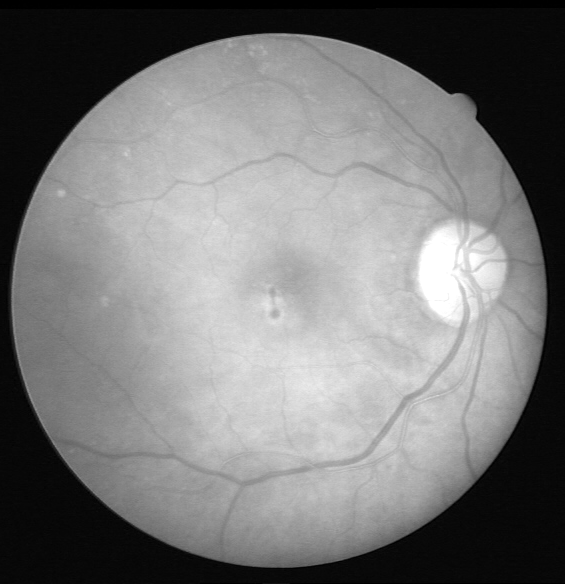
\includegraphics[width=\textwidth]{red.png}
		\caption{Red channel}
		\label{fig:red fundus}
	\end{subfigure}
	%
	\begin{subfigure}[b]{0.3\textwidth}
		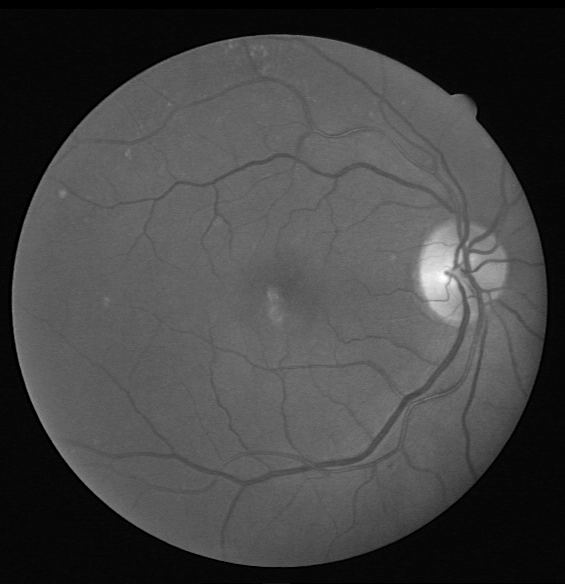
\includegraphics[width=\textwidth]{green.png}
		\caption{Green channel}
		\label{fig:green fundus}
	\end{subfigure}
	\begin{subfigure}[b]{0.3\textwidth}
		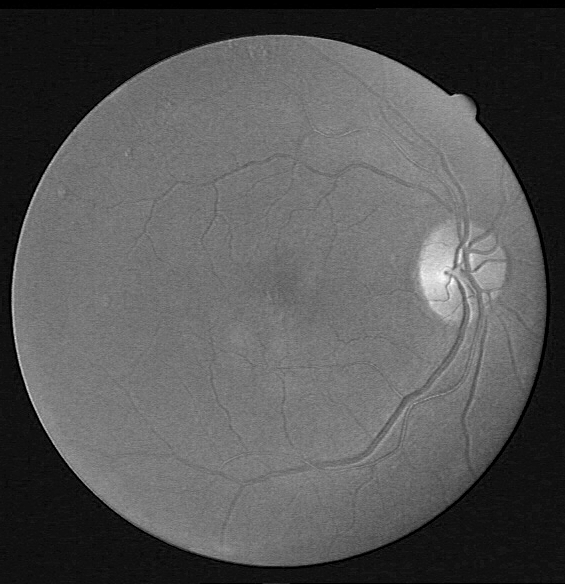
\includegraphics[width=\textwidth]{blue.png}
		\caption{Blue channel}
		\label{fig:blue fundus}
	\end{subfigure}
	\caption[Red, Green, Blue channels of a fundus image]{Different channels of a fundus image showing variation in contrast of blood vessels against background. Green channel shows the maximum contrast in blood vessels and background.}
	\label{fig:fundus image}
\end{figure}

The performance of the proposed vessel segmentation algorithm is evaluated using the segmented vaculature considered as the gold standard and the manually marked segmentations by the human observer.All prior work with which we compare our method, have done a segmentation performance analysis with the manual segmentations provided by the first human observer. Additionally for some of the datasets we have a manual segmentation provided by the second observer which can be used to compare the automated methods to that of manual segmentations.\\

To asses the performance of segmentation methods, various metric have been defined in literature \cite{monteiro2006performance,sharma2001performance}. As reported in prior works,we also compute the performance of our vessel segmentation model defined as, true positives (TP): number of correctly classified vessel pixels; false positives (FP): number of pixels falsely classified as vessels; true negatives(TN): number of correctly classified non-vessel pixels; false negatives(FN): number of pixels falsely classified as non-vessels.\\

Using these metrics we can compute the accuracy (number of TP+TN / total pixels) ,pixel classification sensitivity and specificity. We also calculate the area under curve for receiver operation characteristics and also the AUC under the precision recall curve obtained by varying the threshold value for the segmented images.\\

For a complete assessment of our segmentation model, we perform various experiments. We start by performing the experiment on all the 4 datasets and compute the performance metrics as described above. Next, to test the generalization of our system we do cross training, i.e, training on images from one dataset and prediction on other.

We test the performance of both our models.  	

\section{Vessel Segmentation Assessment}
The proposed models have some input parameters, which need to be evaluated to have the best performance on the models. We start by exploring the various parameters and discuss their effect on our model.\\
\begin{figure}
	\begin{subfigure}[b]{0.45\textwidth}
		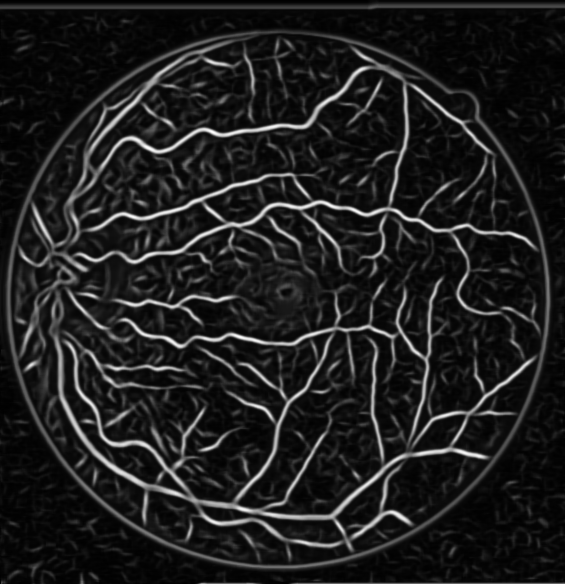
\includegraphics[width=\textwidth]{psize/p10.png}
		\caption{patch size (10,10)}
		\label{fig:p10}
	\end{subfigure}
	%
	\begin{subfigure}[b]{0.45\textwidth}
		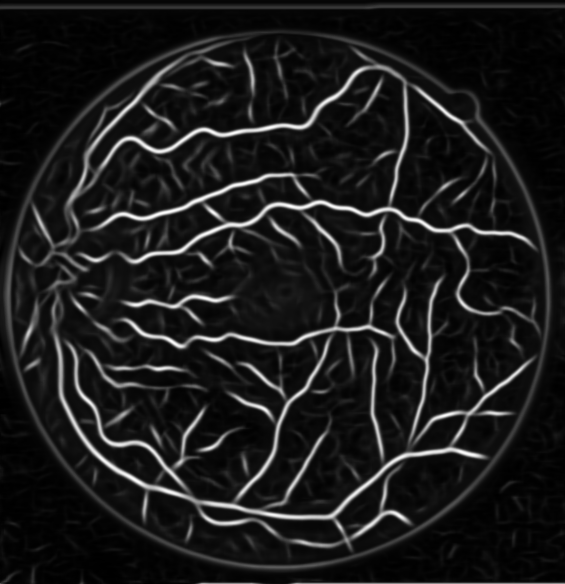
\includegraphics[width=\textwidth]{psize/p15.png}
		\caption{patch size (15,15)}
		\label{fig:p15}
	\end{subfigure}
	
	\begin{subfigure}[b]{0.45\textwidth}
		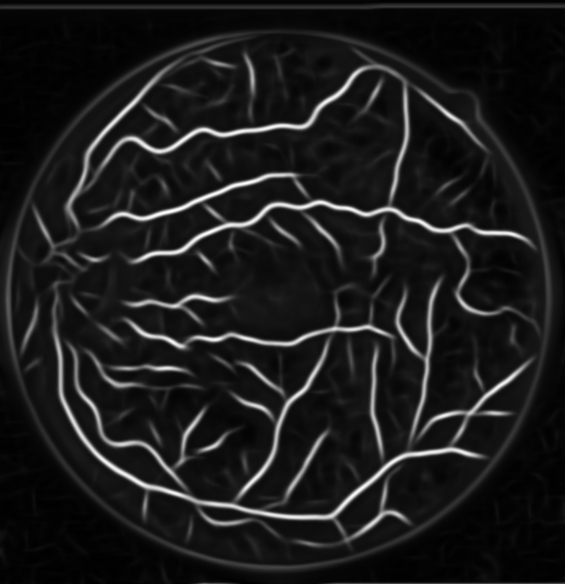
\includegraphics[width=\textwidth]{psize/p21.png}
		\caption{patch size (21,21)}
		\label{fig:p21}
	\end{subfigure}
	\begin{subfigure}[b]{0.45\textwidth}
		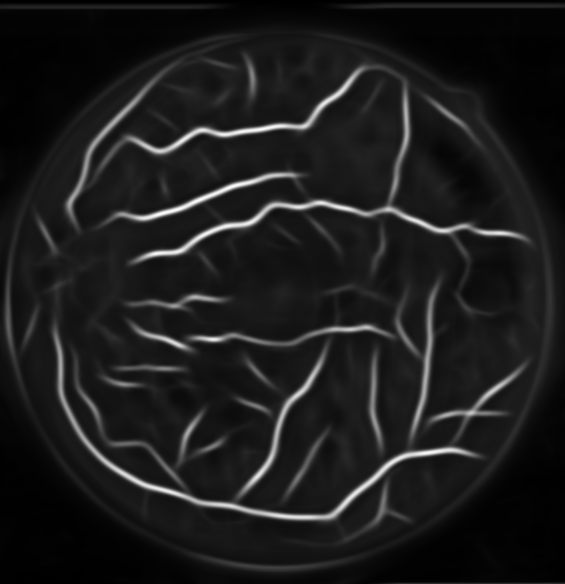
\includegraphics[width=\textwidth]{psize/p33.png}
		\caption{patch size (33,33)}
		\label{fig:33}
	\end{subfigure}
	\caption[Image segmentation using varying patch sizes]{Here we show the effect of varying patch size in our patch based framework. As we increase the patch size, we lose details on thin vessels,but our confidence on thick vessels increases.}
	\label{fig:patch size}
\end{figure}

One of the main parameters of our model is the patch size. As this is a patch based framework the size of patch is very important to us. A small patch size would mean that we may not be able to extract sufficient local information and a bigger patch size would mean that the local structure information would be lost as the patch may constitute multiple local structures. Also as we perform an averaging based reconstruction, the pixel value might get reduced to a very small value during reconstruction due to presence of lot of background pixels.\\ 

We test our model on a multitude of patch size varying from (10,10) to (21,21). The segmentation results for various patch size on an image are show in \ref{fig:patch size}. From the segmentation results, we infer that as the patch size is slowly increased we lose out on the finer details. A larger patch size is able to segment out thick vessels but doesn't perform well on thin vessels. Visually examining the results, patch size of (10,10) and (15,15) give satisfactory results. Figure \ref{fig:patchcompare} shows the ROC curve for DRIVE test set with varying patch size applied with a cluster size K of 1000.\\ 




\begin{figure}
	\centering
	\begin{subfigure}[b]{0.45\textwidth}
		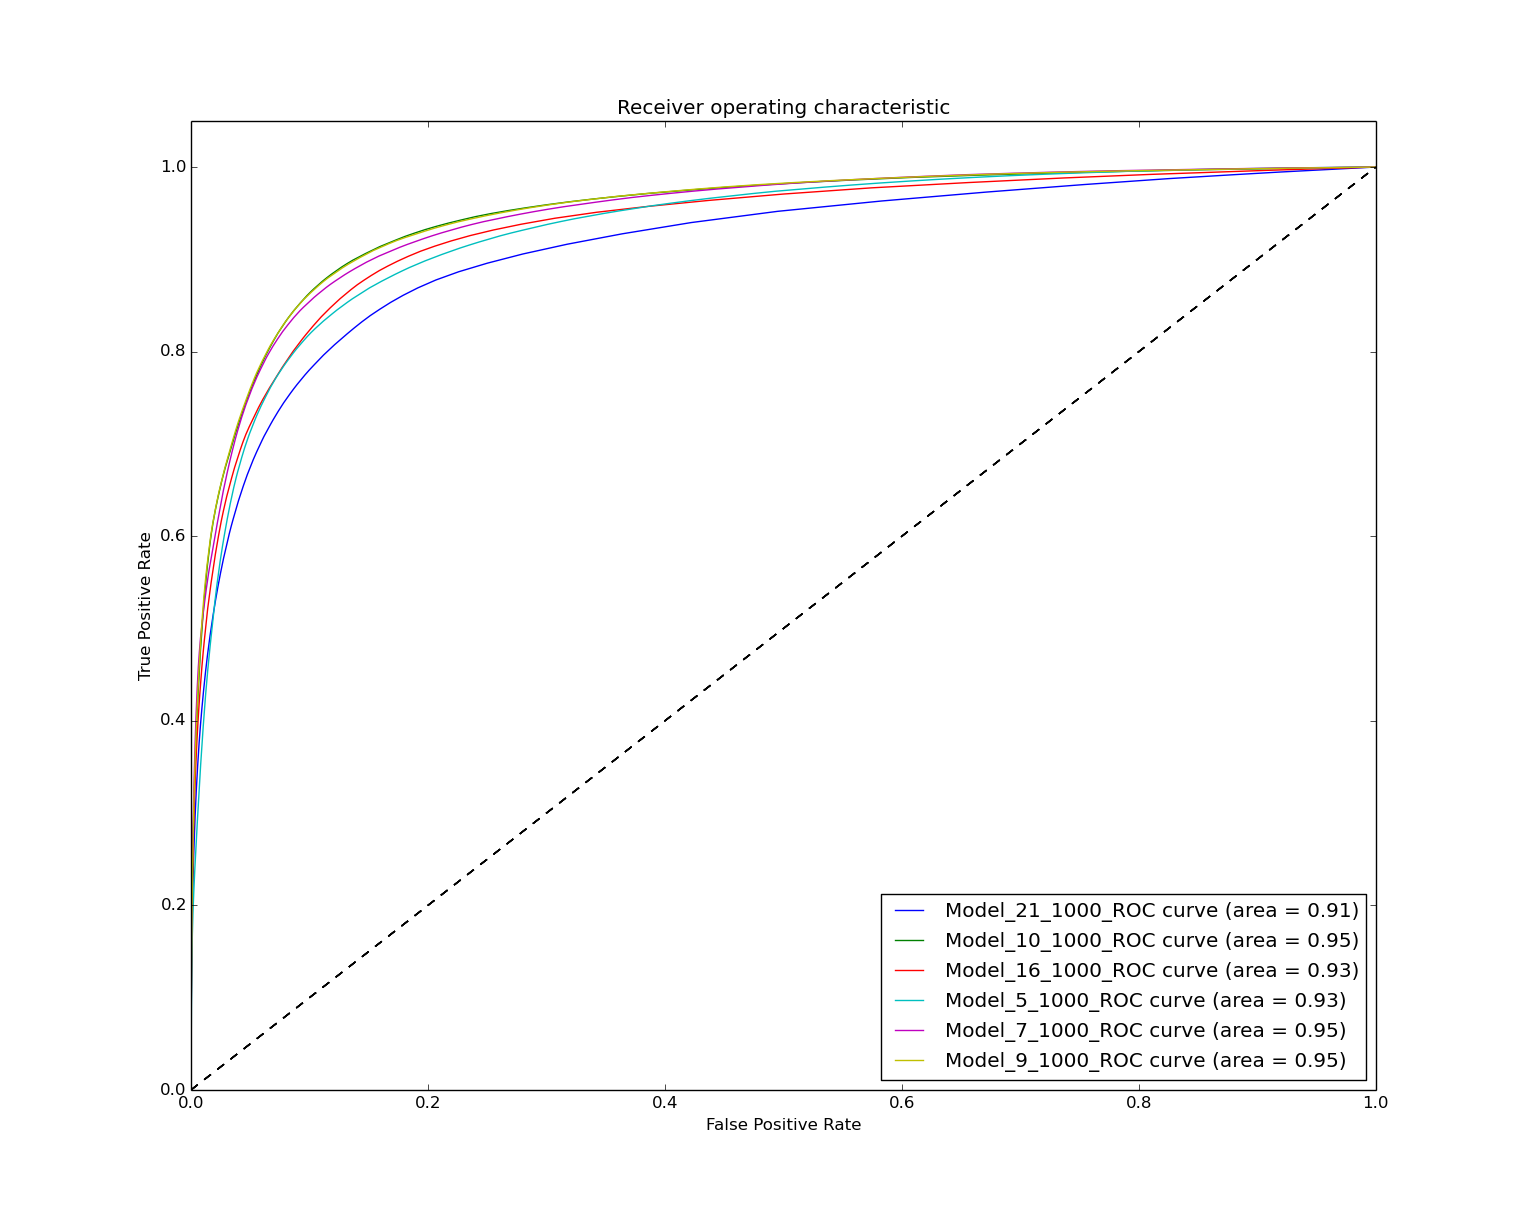
\includegraphics[width=\textwidth]{allmod.png}
		\caption{ROC curve}
		\label{fig:patchcom}
	\end{subfigure}
	\caption[ROC curve with varying patch size]{ROC curve, comparing the performance of our model on DRIVE test set with varying patch sizes.}
	\label{fig:patchcompare}
\end{figure}

The next important parameter in our model is 'K' the number of clusters. The number of clusters forms an important factor in both our models. It determines, the number of local structures we wish to learn from the dataset. Too small a number and we would miss some important local structures present in our data. Increasing the number of clusters beyond a point doesn't add any benefit, but might increase the time complexity. In the dictionary learning model, the number of clusters in general should be larger than the dimension of our feature vectors, to learn an overcomplete dictionary. As we can see in figure \ref{fig:ksize}, a small number of cluster size leads to a lot of noise due to mismatch ground truth annotations.

\begin{figure}
	\begin{subfigure}[b]{0.45\textwidth}
		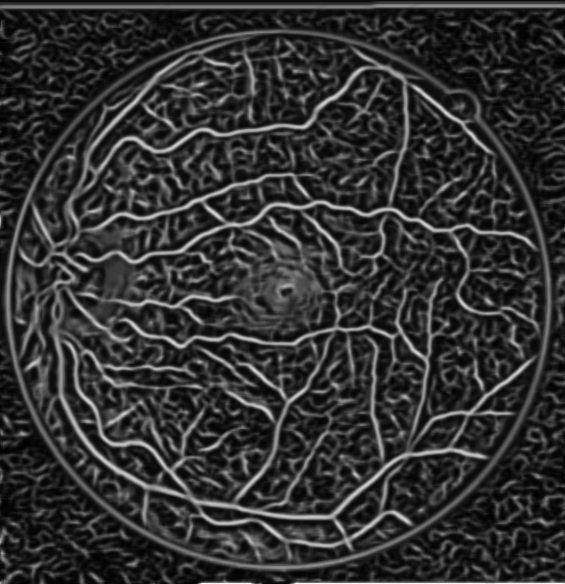
\includegraphics[width=\textwidth]{ksize/k50.png}
		\caption{K=50}
		\label{fig:k50}
	\end{subfigure}
	%
	\begin{subfigure}[b]{0.45\textwidth}
		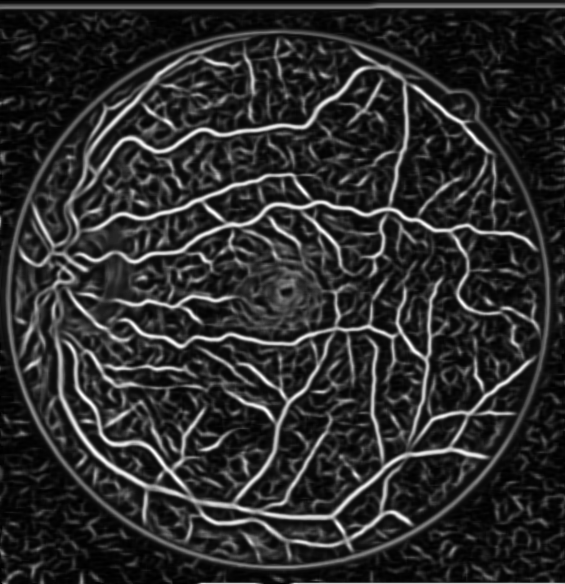
\includegraphics[width=\textwidth]{ksize/k100.png}
		\caption{K=100}
		\label{fig:k100}
	\end{subfigure}
	
	\begin{subfigure}[b]{0.45\textwidth}
		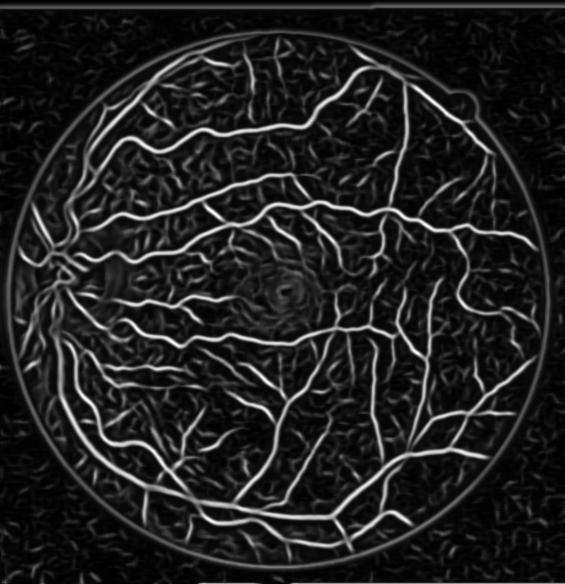
\includegraphics[width=\textwidth]{ksize/k250.png}
		\caption{K=250}
		\label{fig:k250}
	\end{subfigure}
	\begin{subfigure}[b]{0.45\textwidth}
		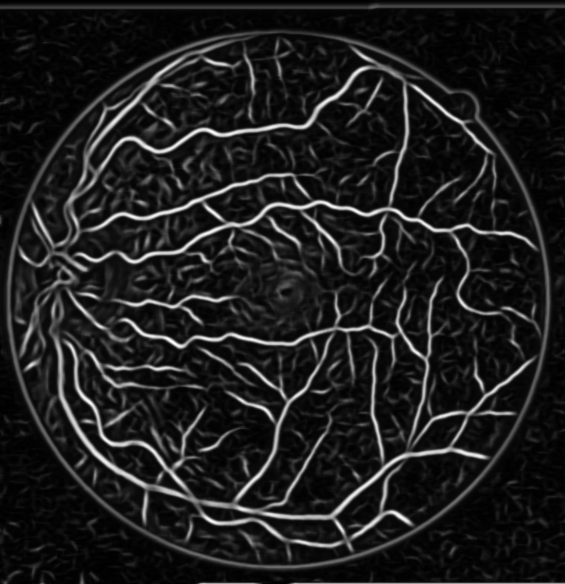
\includegraphics[width=\textwidth]{ksize/k500.png}
		\caption{K=500}
		\label{fig:k500}
	\end{subfigure}
	\caption[Image segmentation using varying the number of clusters]{Here we show the effect of varying the number of clusters in our patch based framework.}
	\label{fig:ksize}
\end{figure}

No we evaluate the segmentation performance of our Cluster Based Common Local Structure classifier (CB-CLS), by training it on the DRIVE train and testing on DRIVE test dataset. The train parameters are set as , patch size of (10,10) with number of clusters K=1000.
The Precision recall curve and receiver operation characteristics for our solution is shown in figure \ref{fig:rocprc}\\

\begin{figure}
	\centering
	\begin{subfigure}[b]{0.45\textwidth}
		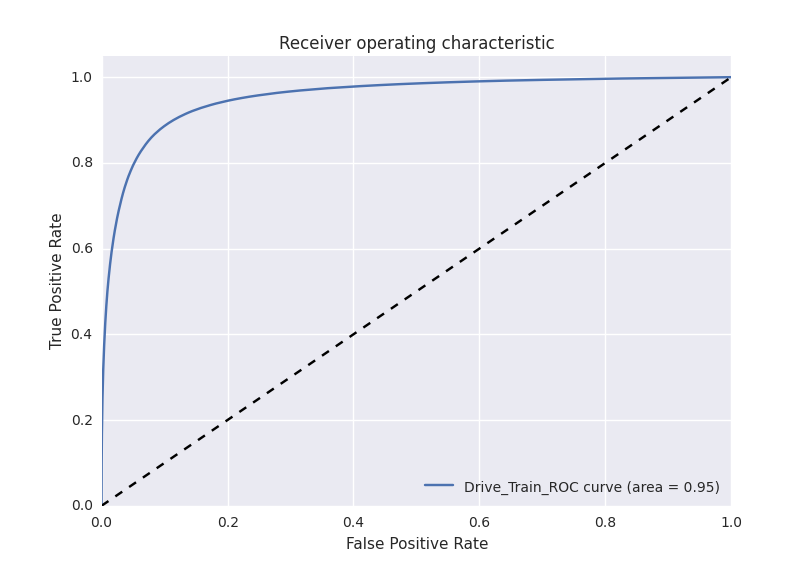
\includegraphics[width=\textwidth]{roc.png}
		\caption{ROC curve}
		\label{fig:roc}
	\end{subfigure}
	\begin{subfigure}[b]{0.45\textwidth}
		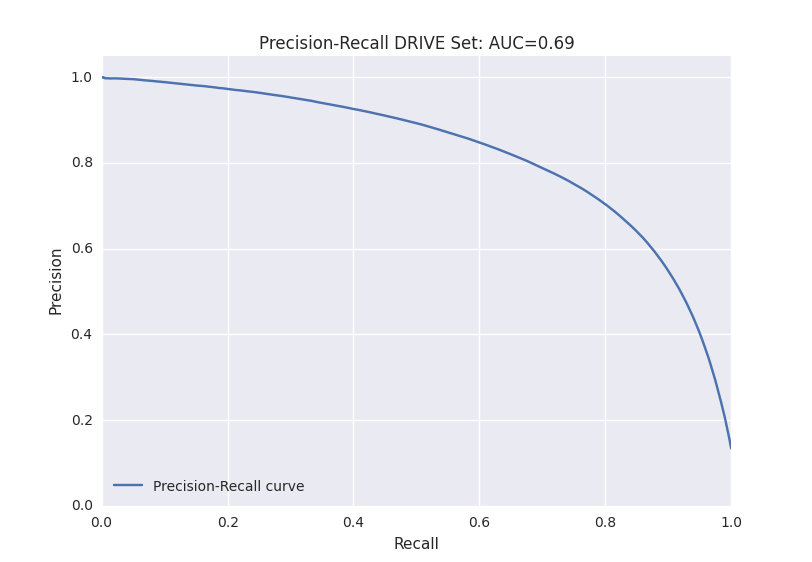
\includegraphics[width=\textwidth]{prc.png}
		\caption{PRC curve}
		\label{fig:prc}
	\end{subfigure}
	\caption[ROC and PRC curve for Cluster Learning based model]{Receiver operation characteristics curve and precision recall curve showing the performance of the Cluster Learning model, compared to ground truth annotation.}
	\label{fig:rocprc}
\end{figure}
\begin{figure}
	\centering
	
	\begin{subfigure}[b]{0.75\textwidth}
		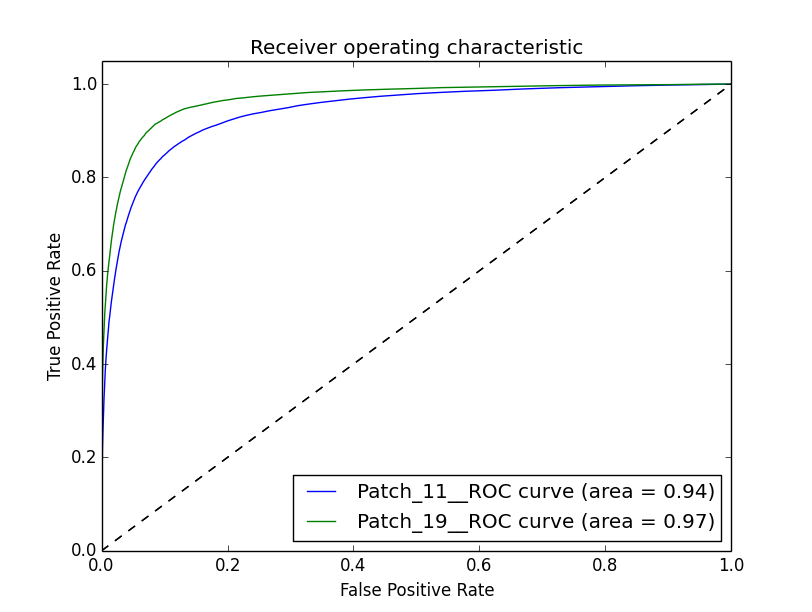
\includegraphics[width=\textwidth]{bestworsecomp.png}
		\caption{ROC Curve}
		\label{fig:bestworse}
	\end{subfigure}
	\caption[ROC curve comparing the best and worse case on DRIVE set]{ROC curve comparing the best and worse case on DRIVE dataset.}
	\label{fig:bestroc}
\end{figure}
\clearpage
A comparison of our model with other methods in literature is shown in figure \ref{fig:compareall}
As we can see, that our cluster learning model has a decent performance and performs better then the structure forests model(SE) proposed by \citep{dollar2013structured}. Also it has a comparable performance to the dictionary learning(DL) based model proposed by \citep{rigamonti2013learning}  and the linear filter model(CS) proposed by \cite{rigamonti2012accurate}.\\

\begin{figure}
	\centering
	
	\begin{subfigure}[b]{0.75\textwidth}
		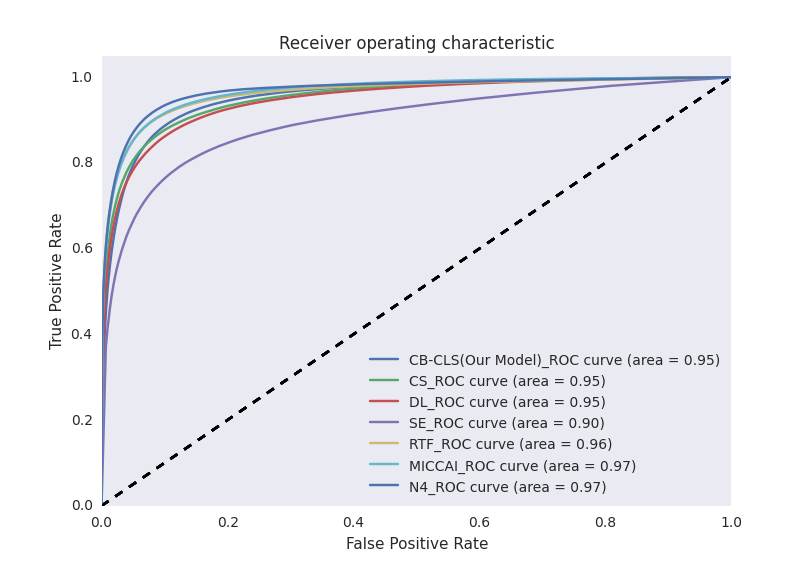
\includegraphics[width=\textwidth]{compareall.png}
		\caption{ROC Curve}
		\label{fig:com}
	\end{subfigure}
	\caption[Results on DRIVE dataset]{We compare our model by testing it on the DRIVE dataset. Results are shown for some of the state-of-art methods in literature. SE is the structured forest model by \citet{dollar2013structured},DL is the dictionary leaned filter model by \citet{rigamonti2013learning}, CS is the linear filter model by \citet{rigamonti2012accurate}, N4 is the CNN-kNN model by \citet{ganin2014n},MICCAI is the method proposed by \citet{becker2013supervised}}
	\label{fig:compareall}

\end{figure}
We then compare the best case and worst case in our model.For the best case the AUC is 0.97 and for the worst case the AUC is 0.94. The best case and worst case segmentations are shown in Figure \ref{fig:bestcase} and figure \ref{fig:worstcase} respectively. Note that the images are not thresholded. The threshold for false positive rate (FPR) of 0.05 is 0.72 as shown in Figure \ref{fig:bestroc} We observe that for the best case scenario, the segmentation is better the near the optic nerve. In case of worst case scenario, we get a very poor segmentation near the optic nerve region.\\

We also compare our model on the stare dataset. As there is no division of dataset provided, to asses the performance of our algorithm we randomly divide the dataset into training and test set with equal number of images. For the stare set we obtain a decent performance with an AUC of 0.96 as shown in figure \ref{fig:stare}
\begin{figure}
	\centering
	
	\begin{subfigure}[b]{0.75\textwidth}
		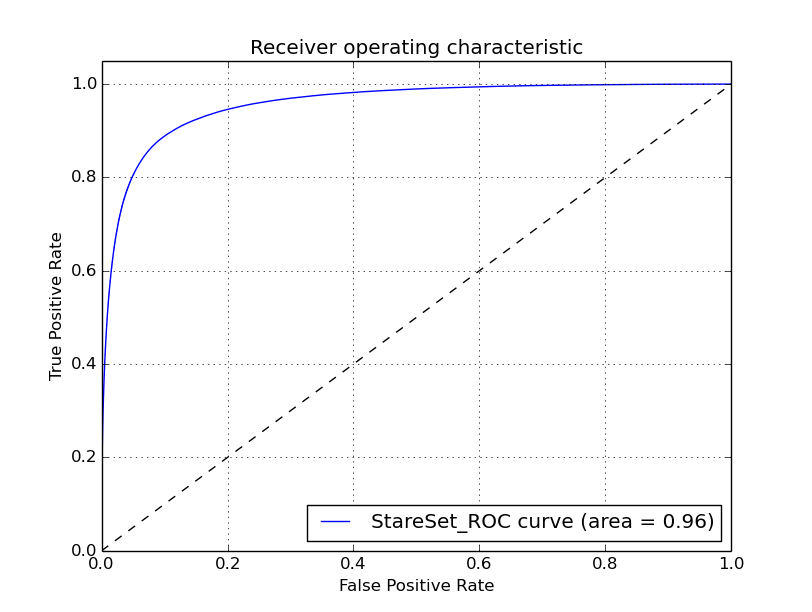
\includegraphics[width=\textwidth]{stare.png}
		\caption{ROC Curve}
		\label{fig:stare1}
	\end{subfigure}
	\caption[ROC curve on a train test split of STARE dataset]{ROC curve for the STARE dataset.}
	\label{fig:stare}
\end{figure}

\begin{figure}
	\centering
	\begin{subfigure}[b]{0.3\textwidth}
		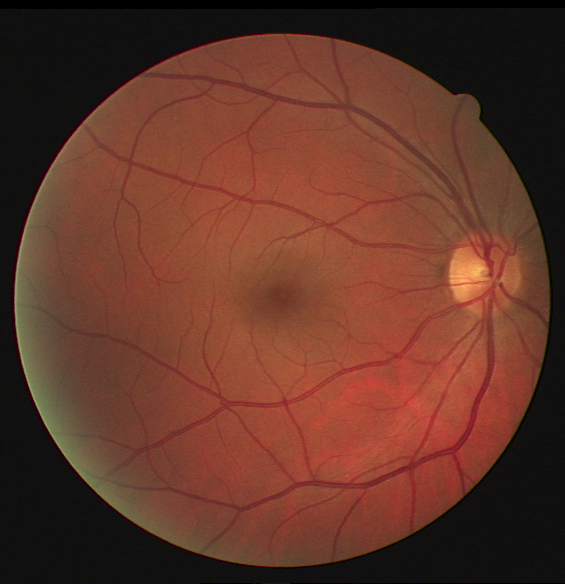
\includegraphics[width=\textwidth]{19.png}
		\caption{Original image}
		\label{fig:191}
	\end{subfigure}
	\begin{subfigure}[b]{0.3\textwidth}
		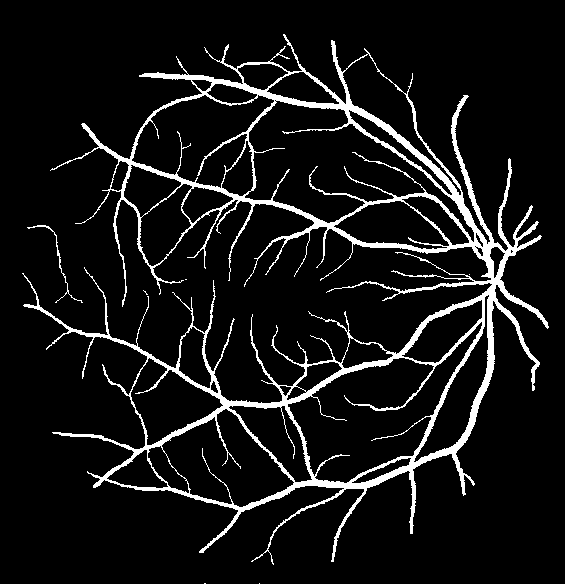
\includegraphics[width=\textwidth]{19m1.png}
		\caption{Ground truth segmentation}
		\label{fig:192}
	\end{subfigure}
	\begin{subfigure}[b]{0.3\textwidth}
		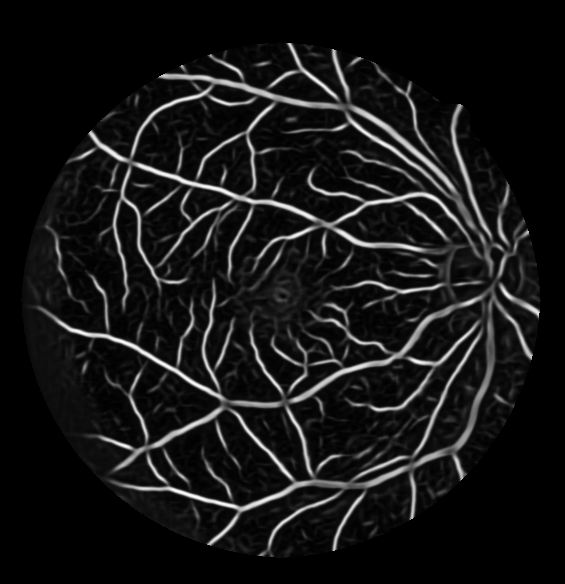
\includegraphics[width=\textwidth]{im19.png}
		\caption{Proposed segmentation}
		\label{fig:193}
	\end{subfigure}
	\caption[Best case on DRIVE test dataset using cluster learning]{This is the best case on DRIVE test dataset, when predicted using the CB-CLS model. The AUC for the proposed solution is 0.97}
	\label{fig:bestcase}
\end{figure}

\begin{figure}
	\centering
	\begin{subfigure}[b]{0.3\textwidth}
		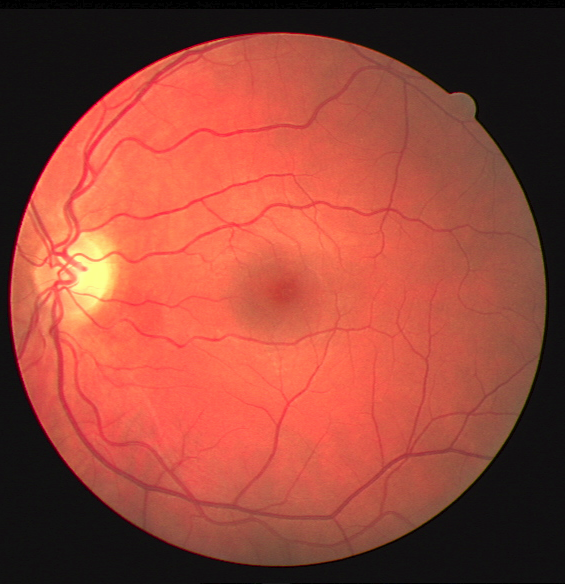
\includegraphics[width=\textwidth]{11.png}
		\caption{Original image}
		\label{fig:111}
	\end{subfigure}
	\begin{subfigure}[b]{0.3\textwidth}
		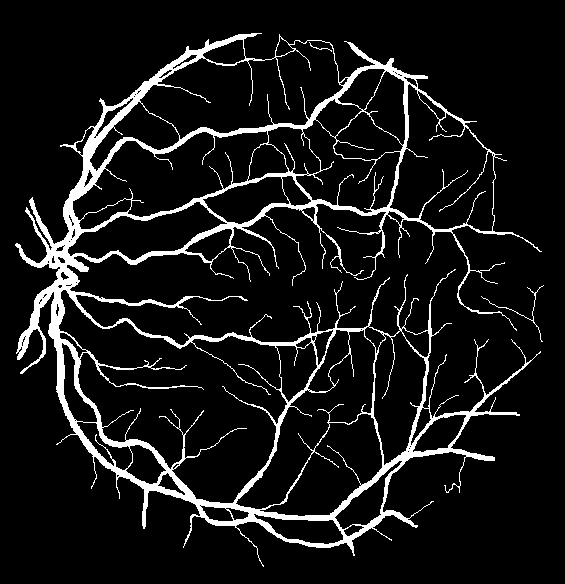
\includegraphics[width=\textwidth]{11m1.png}
		\caption{Ground truth segmentation}
		\label{fig:112}
	\end{subfigure}
	\begin{subfigure}[b]{0.3\textwidth}
		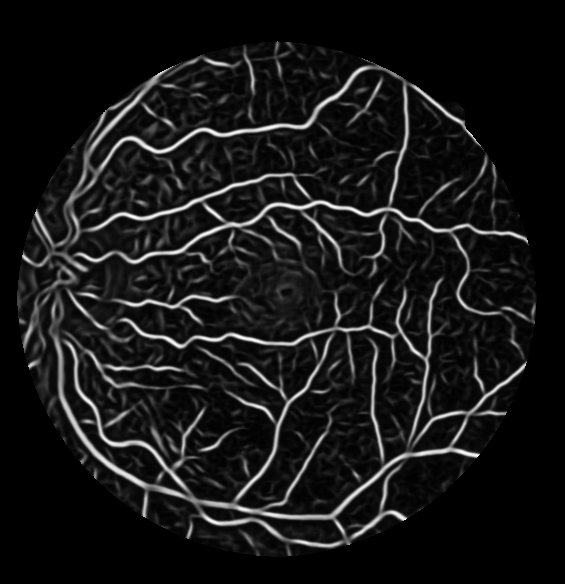
\includegraphics[width=\textwidth]{im11.png}
		\caption{Proposed segmentation}
		\label{fig:113}
	\end{subfigure}
	\caption[Worst case on DRIVE test dataset using cluster learning]{This is the worst case on DRIVE test dataset, when predicted using the CB-CLS model. The AUC for the proposed solution is 0.94}
	\label{fig:worstcase}
\end{figure}

\section{Generalization of the model}\label{sec:generalization}
To check if our model is dependent on the training dataset, we perform an experiment by cross training. We train our model with DRIVE datast, ARIA dataset and CHASEDB dataset, and compute our predictions on the full STARE dataset.
The AUC curves for all the three trainings are shown in figure \ref{fig:comparestare}. We obseve that the performance on the STARE dataset is similar for all the underlying training prcoedures using different datasets. This shows the generalization capabilities of our model. The AUC results for the different training are shown in the table \ref{table:auccompare}

\begin{table}
	\caption{STARE performance for different training sets}
	\centering
	\label{table:auccompare}
	\begin{tabular}{c c  }
		\toprule
		{Datasets} & {AUC}   \\ \hline
		
		DRIVE Train & 0.949 \\
		
		STARE& 0.957 (Training AUC)  \\
		
		ARIA & 0.945 \\
		
		CHASEDB1 & 0.943 \\
		
		\bottomrule
	\end{tabular}
\end{table}


\begin{figure}
	\centering
	\begin{subfigure}[b]{0.45\textwidth}
		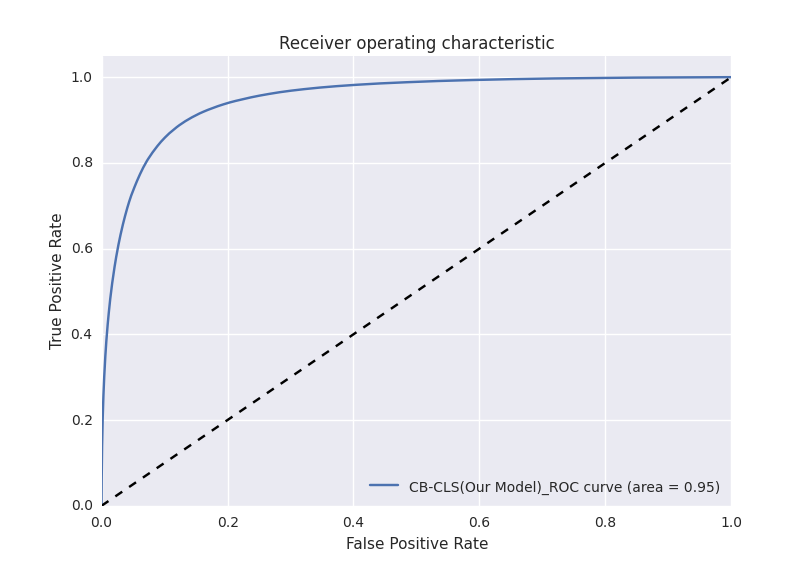
\includegraphics[width=\textwidth]{stare_drive.png}
		\caption{ROC of STARE trained  on DRIVE}
		\label{fig:str}
	\end{subfigure}
	\begin{subfigure}[b]{0.45\textwidth}
		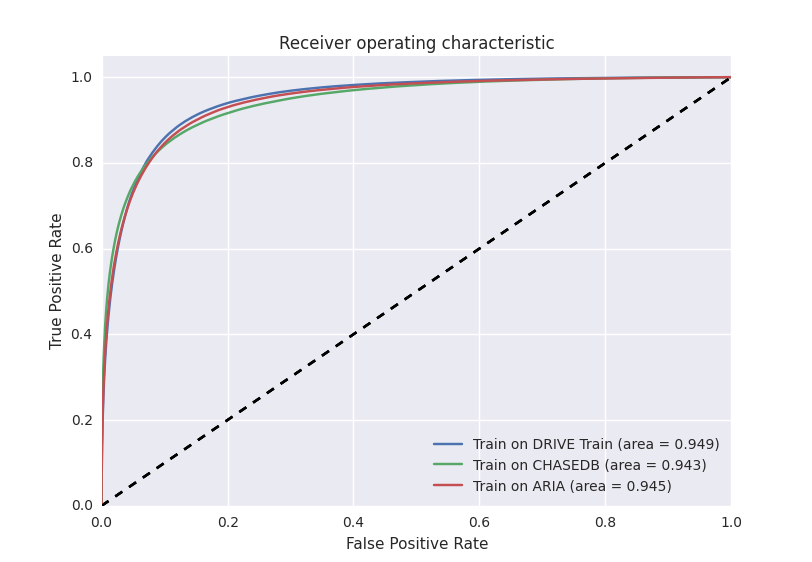
\includegraphics[width=\textwidth]{stare_all.png}
		\caption{ROC for STARE}
		\label{fig:str1}
	\end{subfigure}

	\caption[Cross training comparison for STARE dataset]{We train our classifier on DRIVE,ARIA and CHASEDB dataset and the prediciton are made on STARE set. The ROC curves for all the predictions are shown}
	\label{fig:comparestare}
\end{figure}
\chapter{Conclusion and Future Work}  %Title of the First Chapter

\ifpdf
    \graphicspath{{Chapter4/Figs/Raster/}{Chapter4/Figs/PDF/}{Chapter4/Figs/}}
\else
    \graphicspath{{Chapter4/Figs/Vector/}{Chapter4/Figs/}}
\fi
In this study, we proposed two new learning approaches to solve the problem of vessel segmentation in fundus images.Our models are based on a learning framework from training data.
Our models exploit the presence of frequently occurring basic structures in retinal vessels. In our models, we characterize the presence of structures like edges and straight lines. The model named Cluster Based - Common local structures (CB-CLS), is a partially supervised learning method. We start by learning the common patterns within the raw data by an unsupervised clustering approach and then assigning segmentation maps to them from given segmentation maps.\\
The model works well in predicting thick vessels and parallel vessels. The second model is basically an extension of the first model, where we learn the structures and annotations in a sparse coding dictionary learning framework. Our model, Common Local Structures in Learned dictionaries (CLS-LD), represent each individual patch as a sparse linear combination of dictionary atoms. This helps us to approximate t-junctions and bifurcations in a better way. The preliminary results for our Dictionary learning model were similar to that of the other model. The models requires further tuning and some experiments to verify the capabilities of it. Our methods though very simple, demonstrated good performance compared to the current state-of-art methods.

One of the key contribution in the thesis is a generalizable vessel segmentation model, which is partially independent to the training dataset.Our model has very little dependence on the training data as compared to some other methods whose performance depend on the underlying training data.This comes from the fact that the model exploits the presence of common structures and utilizes them to make structured segmentation prediction at patch level.

Our model though not optimized with speed in mind, has a reasonably fast run time of approximately 4sec per image for an image size of 584 x 565 pixels. This is the total prediction time per image.
With code optimization we can further reduce the run time of our mode. At present we are predicting the patches at all the pixels. By using some initial preprocessing methods, we can get an average segmentation and predict on only the relevant pixels thereby further reducing the run time.\\

The future work would be aimed at extending these methods. Some of the following things we should look into:
\begin{itemize}
	\item Our models do not segment out the very thin vessels perfectly. We should look into extending the model in a way to extract thin vessels. As most of the methods do work very well on the thick vessels,one way to look into it is to have separate models for thin and thick vessels.
	\item The dictionary learning model needs more evaluation. We believe that with better tuning and learning better dictionaries we would be able to estimate the segmentation at crossover regions and bifurcation zones much reliably.
	\item At present we make a dense prediction i.e, we make predictions on all the pixel including the obvious background pixels. By using preprocessing methods or utilizing basic edge detectors, we can detect the points of interest and make prediction much more efficiently.
	\item We should validate our model on other similar problems of vessel segmentation in medical images. 
\end{itemize}





%\include{Chapter6/chapter6}
%\include{Chapter7/chapter7}



% ********************************** Back Matter *******************************
% Backmatter should be commented out, if you are using appendices after References
%\backmatter

% ********************************** Bibliography ******************************
\begin{spacing}{0.9}

% To use the conventional natbib style referencing
% Bibliography style previews: http://nodonn.tipido.net/bibstyle.php
% Reference styles: http://sites.stat.psu.edu/~surajit/present/bib.htm

\bibliographystyle{apalike}
%\bibliographystyle{plainnat} % use this to have URLs listed in References
\cleardoublepage
\bibliography{References/references} % Path to your References.bib file


% If you would like to use BibLaTeX for your references, pass `custombib' as
% an option in the document class. The location of 'reference.bib' should be
% specified in the preamble.tex file in the custombib section.
% Comment out the lines related to natbib above and uncomment the following line.

%\printbibliography[heading=bibintoc, title={References}]


\end{spacing}

% ********************************** Appendices ********************************

\begin{appendices} % Using appendices environment for more functunality

%% ******************************* Thesis Appendix A ****************************
\chapter{How to install \LaTeX} 

\section*{Windows OS}

\subsection*{TeXLive package - full version}
\begin{enumerate}
\item	Download the TeXLive ISO (2.2GB) from\\
\href{https://www.tug.org/texlive/}{https://www.tug.org/texlive/}
\item	Download WinCDEmu (if you don't have a virtual drive) from \\
\href{http://wincdemu.sysprogs.org/download/}
{http://wincdemu.sysprogs.org/download/}
\item	To install Windows CD Emulator follow the instructions at\\
\href{http://wincdemu.sysprogs.org/tutorials/install/}
{http://wincdemu.sysprogs.org/tutorials/install/}
\item	Right click the iso and mount it using the WinCDEmu as shown in \\
\href{http://wincdemu.sysprogs.org/tutorials/mount/}{
http://wincdemu.sysprogs.org/tutorials/mount/}
\item	Open your virtual drive and run setup.pl
\end{enumerate}

or

\subsection*{Basic MikTeX - \TeX~ distribution}
\begin{enumerate}
\item	Download Basic-MiK\TeX (32bit or 64bit) from\\
\href{http://miktex.org/download}{http://miktex.org/download}
\item	Run the installer 
\item	To add a new package go to Start >> All Programs >> MikTex >> Maintenance (Admin) and choose Package Manager
\item	Select or search for packages to install
\end{enumerate}

\subsection*{TexStudio - \TeX~ editor}
\begin{enumerate}
\item	Download TexStudio from\\
\href{http://texstudio.sourceforge.net/\#downloads}
{http://texstudio.sourceforge.net/\#downloads} 
\item	Run the installer
\end{enumerate}

\section*{Mac OS X}
\subsection*{MacTeX - \TeX~ distribution}
\begin{enumerate}
\item	Download the file from\\
\href{https://www.tug.org/mactex/}{https://www.tug.org/mactex/}
\item	Extract and double click to run the installer. It does the entire configuration, sit back and relax.
\end{enumerate}

\subsection*{TexStudio - \TeX~ editor}
\begin{enumerate}
\item	Download TexStudio from\\
\href{http://texstudio.sourceforge.net/\#downloads}
{http://texstudio.sourceforge.net/\#downloads} 
\item	Extract and Start
\end{enumerate}


\section*{Unix/Linux}
\subsection*{TeXLive - \TeX~ distribution}
\subsubsection*{Getting the distribution:}
\begin{enumerate}
\item	TexLive can be downloaded from\\
\href{http://www.tug.org/texlive/acquire-netinstall.html}
{http://www.tug.org/texlive/acquire-netinstall.html}.
\item	TexLive is provided by most operating system you can use (rpm,apt-get or yum) to get TexLive distributions
\end{enumerate}

\subsubsection*{Installation}
\begin{enumerate}
\item	Mount the ISO file in the mnt directory
\begin{verbatim}
mount -t iso9660 -o ro,loop,noauto /your/texlive####.iso /mnt
\end{verbatim}

\item	Install wget on your OS (use rpm, apt-get or yum install)
\item	Run the installer script install-tl.
\begin{verbatim}
	cd /your/download/directory
	./install-tl
\end{verbatim}
\item	Enter command `i' for installation

\item	Post-Installation configuration:\\
\href{http://www.tug.org/texlive/doc/texlive-en/texlive-en.html\#x1-320003.4.1}
{http://www.tug.org/texlive/doc/texlive-en/texlive-en.html\#x1-320003.4.1} 
\item	Set the path for the directory of TexLive binaries in your .bashrc file
\end{enumerate}

\subsubsection*{For 32bit OS}
For Bourne-compatible shells such as bash, and using Intel x86 GNU/Linux and a default directory setup as an example, the file to edit might be \begin{verbatim}
edit $~/.bashrc file and add following lines
PATH=/usr/local/texlive/2011/bin/i386-linux:$PATH; 
export PATH 
MANPATH=/usr/local/texlive/2011/texmf/doc/man:$MANPATH;
export MANPATH 
INFOPATH=/usr/local/texlive/2011/texmf/doc/info:$INFOPATH;
export INFOPATH
\end{verbatim}
\subsubsection*{For 64bit OS}
\begin{verbatim}
edit $~/.bashrc file and add following lines
PATH=/usr/local/texlive/2011/bin/x86_64-linux:$PATH;
export PATH 
MANPATH=/usr/local/texlive/2011/texmf/doc/man:$MANPATH;
export MANPATH 
INFOPATH=/usr/local/texlive/2011/texmf/doc/info:$INFOPATH;
export INFOPATH

\end{verbatim}



%\subsection{Installing directly using Linux packages} 
\subsubsection*{Fedora/RedHat/CentOS:}
\begin{verbatim} 
sudo yum install texlive 
sudo yum install psutils 
\end{verbatim}


\subsubsection*{SUSE:}
\begin{verbatim}
sudo zypper install texlive
\end{verbatim}


\subsubsection*{Debian/Ubuntu:}
\begin{verbatim} 
sudo apt-get install texlive texlive-latex-extra 
sudo apt-get install psutils
\end{verbatim}

%% ******************************* Thesis Appendix B ********************************

\chapter{Installing the CUED class file}

\LaTeX.cls files can be accessed system-wide when they are placed in the
<texmf>/tex/latex directory, where <texmf> is the root directory of the user’s \TeX installation. On systems that have a local texmf tree (<texmflocal>), which
may be named ``texmf-local'' or ``localtexmf'', it may be advisable to install packages in <texmflocal>, rather than <texmf> as the contents of the former, unlike that of the latter, are preserved after the \LaTeX system is reinstalled and/or upgraded.

It is recommended that the user create a subdirectory <texmf>/tex/latex/CUED for all CUED related \LaTeX class and package files. On some \LaTeX systems, the directory look-up tables will need to be refreshed after making additions or deletions to the system files. For \TeX Live systems this is accomplished via executing ``texhash'' as root. MIK\TeX users can run ``initexmf -u'' to accomplish the same thing.

Users not willing or able to install the files system-wide can install them in their personal directories, but will then have to provide the path (full or relative) in addition to the filename when referring to them in \LaTeX.



\end{appendices}

% *************************************** Index ********************************
\printthesisindex % If index is present

\end{document}
